\section{Durchführung}
\label{sec:Durchführung}

Um das Trägheitsmoment bestimmter Körper zu berechnen, wird eine Drillachse verwendet.
Dabei werden die Körper auf einer drehbaren Achse befestigt, welche über eine Spiralfeder mit dem Rahmen verbunden ist.
Um zunächst die Winkelrichtgröße und das Eigenträgheitsmoment der Drillachse zu berechnen,
wird eine nahezu masselose Stange auf der Achse befestigt. 
Dann wird eine Federwaage senkrecht zur Stange eingehackt,da sonst eine ungenaue Kraft angezeigt wird, und um bestimmte Winkel ausgelenkt.
Die gemessene Kraft, der Radius und der Winkel werden notiert und die Messung wird 10 mal durchgeführt.

Auf die masselose Stange werden in gleichem Abstand zwei Gewichte angebracht, und das System wird zum Schwingen gebracht.
Die Schwingungsdauer wird für 10 verschiedene Abstände gemessen.

Zur Trägheitsmoment-Bestimmung einer Kugel und eines Zylinders, werden diese auf der Achse befestigt, und ausgelenkt.
Wieder wird die Schwingungsdauer gemessen, diesmal 5 mal. 

Auf gleiche Weise wird die Schwingungsdauer einer Holzpuppe in zwei verschiedenen Stellungen gemessen.

\begin{figure}[H]
  \centering
  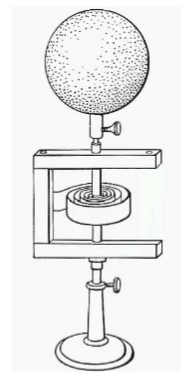
\includegraphics[height=8cm]{Drillachse.PNG}
  \caption{Die Drillachse.}
  \label{fig:drill}
\end{figure}

